% !TEX TS-program = xelatex
% The "real" document content comes below...
% !TEX TS-program = xelatex
% !TEX encoding = UTF-8 Unicode
% \ProvidesClass{classname}[2017/02/27 notes]
\documentclass[10pt]{article}%__________________________________________________________________Page geometry
% \usepackage[letterpaper,margin=0.6in,marginratio=3:5,twoside]{geometry}
\usepackage[a4paper,margin=15mm,marginratio=3:5,twoside]{geometry}
% \usepackage[a5paper,margin=13mm]{geometry}
%\usepackage[letterpaper,margin=0.6in,marginratio=3:5,twoside]{geometry}
% \usepackage[paperwidth=5.5in, paperheight=8.5in, margin=13mm]{geometry}
% \usepackage{relsize}
% \relscale{0.3} % or whatever scaling is desired
%\geometry{landscape} % sets the page to landscape orientation

%\usepackage{ulem}
% \usepackage{fancyhdr} % This should be set AFTER setting up the page geometry
%\pagestyle{fancyplain} % options: empty , plain , fancy
%_____________________________________________________________________MATH STUFF
\usepackage{amsmath,amssymb,amsopn}% read amsldoc.pdf for more details
\usepackage{fontspec}
\usepackage{unicode-math}
%\DeclareMathOperator{\}{}
\DeclareMathOperator{\arccot}{arccot}
\DeclareMathOperator{\arcsec}{arcsec}
\DeclareMathOperator{\arccsc}{arccsc}
\DeclareMathOperator{\sech}{sech}
\DeclareMathOperator{\csch}{csch}
\DeclareMathOperator{\arcsinh}{arcsinh}
\DeclareMathOperator{\arccosh}{arccosh}
\DeclareMathOperator{\arctanh}{arctanh}
\DeclareMathOperator{\arccoth}{arccoth}
\DeclareMathOperator{\arcsech}{arcsech}
\DeclareMathOperator{\arccsch}{arccsch}
%\DeclareMathOperator{\min}{min}
%\DeclareMathOperator{\max}{max}
%____macros to make quick note taking easier all escapes under 3 chars
\def\t{\text }
\def\parti{\partial}
\def\o{\over}
\def\({\left( }
\def\){\right) }
\def\[{\left[ }
\def\]{\right] }
% \def\l{\left. }
% \def\r{\right. }
%\usepackage{leqno}
%__________________________________________________________________Font settings
% \usepackage[scaled=.92]{helvet}
% \usepackage{times}
% \usepackage{morefloats}
\usepackage{xcolor}
\usepackage{titlesec}
% \defaultfontfeatures{Ligatures=TeX}
\setsansfont{NotoSans-Light.ttf} % Set sans serif font
% \setsansfont{DejaVu Sans, ExtraLight} % Set sans serif font
% \setsansfont{DejaVu Sans ExtraLight}
% [    Extension = .ttf,
%    UprightFont = *,
%       BoldFont = *-Bold,
%     ItalicFont = *-Italic,
% BoldItalicFont = *-BoldItalic,
% ]
% \setmainfont{Latin Modern Math} % Set serifed font
% \setmainfont{DejaVu Math TeX Gyre} % Set serifed font
\setmainfont{XITS} %#/usr/share/texlive/texmf-dist/fonts/opentype
[    Extension = .otf,
   UprightFont = *-Regular,
      BoldFont = *-Bold,
    ItalicFont = *-Italic,
BoldItalicFont = *-BoldItalic,
]
\setmathfont{XITSMath-Regular}
[    Extension = .otf,
      BoldFont = XITSMath-Bold,
]
% \setmathfont{Latin Modern Math} % Set serifed font

% Define light and dark Microsoft blue colours
\definecolor{MSBlue}{rgb}{.204,.353,.541}
\definecolor{MSLightBlue}{rgb}{.31,.506,.741}
\definecolor{PitchBlack}{rgb}{.0,.0,.0}

% Define a new fontfamily for the subsubsection font
% Don't use \fontspec directly to change the font
% \newfontfamily\subsubsectionfont[Color=MSLightBlue]{DejaVu Math TeX Gyre}
% Set formats for each heading level

\titleformat*{\section}{\Large\bfseries\sffamily\color{PitchBlack}}
\titleformat*{\subsection}{\Large\bfseries\sffamily\color{PitchBlack}}
\titleformat*{\subsubsection}{\Large\bfseries\sffamily\color{PitchBlack}}
% \titleformat*{\subsection}{\large\bfseries\sffamily\color{MSLightBlue}}
% \titleformat*{\subsubsection}{\itshape\subsubsectionfont}

%______________________________Multicol http://tex.stackexchange.com/a/3987/1244
\usepackage{multicol}
\usepackage{ifthen}
% \let\oldsection\section
% \renewcommand*{\section}[1]{%
%     \ifthenelse{\equal{\@currenvir}{multicols}}{\end{multicols}}{}
%     \ifthenelse{\thesection = 0}{}{\end{multicols}}%
%     \begin{multicols}{2}[\oldsection{#1}]}
% \let\oldsubsection\subsection
% \renewcommand*{\subsection}[1]{%
%     \ifthenelse{\thesubsection = 0}{}{\end{multicols}}%
%     \begin{multicols}{2}[\oldsubsection{#1}]}
% \let\oldend\enddocument
% \renewcommand*{\enddocument}{\end{multicols}\oldend}


\usepackage{pst-node}% http://ctan.org/pkg/pst-node
\usepackage{tabu}
\usepackage{natbib}
\usepackage{graphicx}
%\usepackage{hyperref}
\usepackage[colorlinks=true,linkcolor=black,anchorcolor=black,citecolor=black,filecolor=black,menucolor=black,runcolor=black,urlcolor=black]{hyperref}%\usepackage{textcomp}
\title{${2.267061 \text{grams} \over \text{1.39}\times 10^{24}} \approx {{c ~ T_{SI}\over L_F}M_F \over \text{1.39}\times 10^{24}}=\sqrt{k_e^2~q_e^4~T \over c~G~M~L^2}= \sqrt{c ~\alpha^2 ~ \hbar^2 ~T\over G~M~L^2}=M_F$ }
\author{\copyright Roy Pfund\thanks{e-mail: r0ypfund@gm41l.c0m} ~(CC BY-NC-SA 4.0) 2022\\
\url{https://creativecommons.org/licenses/by-nc-sa/4.0/}}
%\date{} % Activate to display a given date or no date (if empty), otherwise the current date is printed
\begin{document}
\bibliographystyle{plainnat}
%\maketitle
%\begin{multicols}{2}
\maketitle
%% Abstract section.
%\begin{abstract}
%testing
%\end{abstract}
%\end{multicols}
%-------------Abstract--------------
%\begin{multicols}{2}
\begin{multicols}{2}
Some CFD software uses planck units to reduce computation by reducing the billions of multiplications of $k_b$; we should care about people as much as machines and reduce the constants people have to know.~$M_F^{W}L_F^{X}T_F^{Y}Q_F^{Z}=$% (besides masses of subatomic particles).
%Using ${q_e \over coulomb}{kg\cdot m^2 \over s^2}=eV=1.602176634×10^{-19} J =$ the ElectronVolt; units of $\text{Mass}={eV \over c^2}$, $\text{Length}={\hbar c \over eV}$, or $\text{Time}={\hbar \over eV}$ can be constructucted.  Maybe we can do better:
%$$
%%\text{Pfund Mass} = M_F^{1}\qquad
% {\hbar \over c M_F} = L_F = {\hbar ~ c \over E_F};\qquad
%{\hbar \over c^2 M_F} = T_F = {\hbar \over E_F};\qquad
%q_e = Q_F
%$$
$${\( \sqrt{c ~\alpha^2 ~ \hbar^2 ~T\over G~M~L^2}\)}^W {\({G \over c^2 }M_F{M~L^2 \over \alpha^2 \hbar ~T }\)}^X {\({G \over c^3 }M_F{M~L^2 \over \alpha^2 \hbar ~T }\)}^Y {\(q_e\)}^Z$$
\begin{multicols}{2}[\setlength{\columnseprule}{0pt}]\noindent\begin{align*}
k_e = ~\alpha &~M_F^{1}L_F^{3}T_F^{-2}Q_F^{-2}\\
\mu _0 = ~\alpha~4~\pi &~M_F^{1}L_F^{1}Q_F^{-2}\\
\epsilon _0 = ~{1 \over \alpha~4~\pi} & ~M_F^{-1}L_F^{-3}T_F^{2}Q_F^{2}\\% ={1 \over \mu _0 c^2}
%$${\alpha ^2~m_e~c~\over~4~\pi ~\hbar~ L_F}={R_\infty\over L_F}={\alpha ^2~m_e~\over~4~\pi~ L_F}{L_F\over T_F}{T_F \over M_F~L_F^2}={\alpha ^2~m_e\over~4~\pi~M_F~L_F^2}$$
R_\infty = {m_e\over M_F}{\alpha ^2\over~4~\pi}&~L_F^{-1}
%constant = ~1 ~&M_F^{}L_F^{}T_F^{}Q_F^{}\\
%constant = ~1 ~&M_F^{}L_F^{}T_F^{}Q_F^{}\\
\end{align*}\noindent\begin{align*}
%\text{Pfund Mass} = ~1 &~M_F^{1}\\
%{\hbar \over c M_F} = ~1 &~L_F\\
%{\hbar \over c^2 M_F} = ~1&T_F\\
%q_e = ~1 &~Q_F\\
\hbar = ~1 & ~M_F^{1}L_F^{2}T_F^{-1}\\
c = ~1 & ~L_F^{1}T_F^{-1}\\
N_A = ~1 &\text{**}\\
M_F~ c^2 =E_F = ~1 & ~M_F^{1}L_F^{2}T_F^{-2}\\
{2~\pi~\hbar \over c ~ q_e}=k_b = ~2\pi & ~M_F^{1}L_F^{1}Q_F^{-1}
%constant = ~1 ~&M_F^{}L_F^{}T_F^{}Q_F^{}\\
%constant = ~1 ~&M_F^{}L_F^{}T_F^{}Q_F^{}\\
%G = ~{10^{-14} Q^4_F\over M_F T_F} ~&M_F^{3}L_F^{-1}T_F^{-2}Q_F^{}\\
\end{align*}\noindent\end{multicols}\noindent
%\begin{align*}
%{\hbar \over c^2 M_F}~{c ~ T_{SI}\over L_F} &=~T_F~D_C &= ~1 \text{Second} \\
%{\hbar \over c M_F}~{{c ~ T_{SI}\over L_F}\over 299792458} &=~L_F~{D_C\over 299792458}  &= ~1 \text{Meter}\\
%{c ~ T_{SI}\over L_F}~q_e&= ~Q_F~D_C &\approx~222702.257\text{Coulombs} \\
%%\text{Pfund Mass}~{c ~ T_{SI}\over L_F} &=\vcenter{\hbox{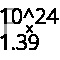
\includegraphics[width=1.6em]{P.ps}}}=~M_F~D_C &\approx 2.267061 \text{grams}
%\text{Pfund Mass}~{c ~ T_{SI}\over L_F} &=~M_F~D_C &\approx 2.267061 \text{grams}
%\end{align*}
\noindent\section {Dimensionality}Stoney-Mass $M_{{\text{S}}} = \sqrt{\hbar ~ \alpha ~c \over G}$ units are correct, but with $M_F = M_S \sqrt{\hbar \alpha}$ alone gives correct arithmetic;
 for all the equations above to not only work arithmeitc wise, $\sqrt{T \over M^{1}L^{2}}$ is needed to cancel any wrong units put into $M_F$ from $\hbar$. M, L, and T with no subscripts are meant to mean from whichever unit system you are converting from or currently using, in this case; SI units 1kg, 1m, and 1s respectively.
%$$\hbar~\alpha^2 = {10^{-14} Q^4_F\over M_F T_F} ={G \over ~M_F^{3}L_F^{-1}T_F^{-2}Q_F^{0}}$$
$\sqrt{T \over M^{1}L^{2}}$ reappears in the solution for $G$. However $G$ is wrong to begin with, because with Relativity it doesn't really exist, as it is the curvature of space time.
$$\alpha^2\hbar= \alpha^2 {M_F^{}L_F^{2} \over T_F} ={G \over ~M_F^{3}L_F^{-1}T_F^{-2}}$$

%$${\psDefBoxNodes{n2}{\mu _{0}} \over 2} ={\psDefBoxNodes{n4}{h ~ \alpha} \over c ~ q_e^2}; \hspace{0.5em} {\psDefBoxNodes{n5}{h ~ \alpha} \over c~ q_e^2}{ c^2 \over 2\pi }=k_e={1\over 4 \pi \epsilon _0};\hspace{0.5em} \epsilon _0 ={1 \over \mu _0 c^2}
%\psset{nodesep=3pt,arcangle=35}
%\ncarc{<->}{n2:tC}{n4:tC}
%\ncarc{<->}{n4:tC}{n5:tC}
%$$
How the constants below are derived/involved with $\alpha$, it seems to only make sense, for it be the only number we need for our unit system.
$${{h ~ \alpha} \over c~ q_e^2}{ 2 c^2 \over 4\pi }={ \mu _{0}~c^2 \over 4\pi }={1\over 4 \pi \epsilon _0}=k_e;\hspace{0.5em}{{\mu _{0} }\over 2}{c ~ q_e^2 \over 2~\pi ~\hbar}=\alpha $$
%$$ %{\mu _{0} ~c ~ q_e^2 \over 2 ~ h} 
%{{\mu _{0} }\over 2}{c ~ q_e^2 \over 2~\pi ~\hbar} 
%= {2 ~\pi~10^{−7} ~299792458 ~ {(1.602176634 × 10^{-19})}^2   \over 6.62607015 × 10^{-34}} = \alpha $$
$= 0.00729735257$ ``It has been a mystery ever since it was discovered more than fifty years ago, and all good theoretical physicists put this number up on their wall and worry about it.''\citep[p. 129]{feynman1985qed}. %$\hspace{2.5em} k_e ={10^{−7} ~c^2 }{T^2 \over L^2}{M~L^3 \over T^2~Q^2}$
% $k_e ={h ~ \alpha \over c~ q_e^2}{ c^2 \over 2\pi }={10^{−7} ~c^2 }{T^2 \over L^2}{M~L^3 \over T^2~Q^2}$
% — Richard P. Feynman (1985). QED: The Strange Theory of Light and Matter. Princeton University Press. p. 129. ISBN 978-0-691-08388-9.
%\subsection{Vacuum permittivity \& permeability}
%$$2~\pi ~10^{−7} =  {h ~ \alpha \over c ~ q_e^2} {Q^2 \over M ~ L} = {Q^2 \over M ~ L}  {\mu _{0} \over 2} \qquad {\mu _{0} \over 2}{c ~ q_e^2 \over h} = \alpha$$
%\columnbreak
%$$\sqrt{{T_F \over M_F^{}L_F^{2} } {G \over ~M_F^{3}L_F^{-1}T_F^{-2}}}= \alpha$$
\section {Speed of Sound = $c_0$}
Given $c_0 =\sqrt{γ_0  N_A k_B K \over MolarMass}$ and $39.947 g~mol^{-1} =$ molar mass of the argon gas from the experiment measuring $c_0$ in a purifed isotope of argon gas at the Triple-Point of water = 273.16K \citep{Podesta_2013} Where $U_F = {M~L^2 \over k_b~T^2}$, $K = {Kelvin\over U_F}U_F$, and $γ_0 = 5/3$ for monotonic gases. Let's see how this matches up with the $c_0^2 = 94756.245 m^2 s^{-2}$ from the experiment in 2013.\\e.g. on how to correct $N_A$ being based on the Dalton = ${1 \over 12}$ the mass of Carbon isotope $C^{12}$ over to $M_F$ 
\begin{align*}
&\text{**adjusted argon gas molar mass}= 40.671M_F= {39.947 kg \over M_F ~ N_A }\\
&c_0 =\sqrt{{5\over 3}  ~N_A ~ k_B  ~{273.16 Kelvin\over U_F} ~U_F \over 40.671M_F}=307.701 m s^{-1}\approx \sqrt{c_0^2}
\end{align*}
\section{Time is On Our Side(\& Distance)}
With a Sympathetic Constant $=D_C=$ light-second / $L_F$ to save our wallets, watches, measuring wheels, and road signage we can still use existing definitions of distance and time. 
Perhaps one day for the sake of simplicity, Bureau international des poids et mesures might redefine the second and meter such that $D_C$ is exactly $1.39\times 10^{24}$ rather than approx. 5 almost 6 nines.
$${1.3899982\times 10^{24}  \approx {c ~ T_{SI}\over L_F} =D_C \over1.39\times 10^{24}}=0.999998675$$
\section{There and back again}
%${\({c{s\over m}}\)}^{}=299792458$\\
%${D_C}^{-1}{\({c{s\over m}}\)}^{-1}$\\
%4.4903002 e-6 $D_C q_e$ per 1 Coulombs\\ 441.09973 $D_C M_F$ per 1 Kg\\
Calibrating scales to $D_C M_F\approx 2.267061 \text{grams} $ and ammeter to $D_C q_e\approx 222702.26 \text{ Coulombs}$ will result in~$M_F^{W}L_F^{X}T_F^{Y}Q_F^{Z}=$\\
%Calibrating scales to $D_C M_F\approx {Kg \over 441.09973}$ and ammeter to $D_C q_e \approx {Coulomb \over 4.4903002e-06}$ will result in~$M_F^{W}L_F^{X}T_F^{Y}Q_F^{Z}=$\\
${\(  {p~=~D_C M_F \over \text{1.39}\times 10^{24}}\)}^W {\({299792458 \text{Meters}\over \text{1.39}\times 10^{24}}\)}^X {\({1 \text{Second}\over \text{1.39}\times 10^{24}}\)}^Y {\({q~=~D_C q_e\over \text{1.39}\times 10^{24}}\)}^Z$
\begin{multicols}{2}[\setlength{\columnseprule}{0pt}]\noindent\begin{align*}
\mu _0 &= ~\alpha~4~\pi{\({c{s\over m}}\)}p^{1}m^{1}q^{-2}\\
\epsilon _0 &= ~{1 \over \alpha~4~\pi}{\({c{s\over m}}\)}^{-3} p^{-1}m^{-3}s^{2}q^{2}\\% ={1 \over \mu _0 c^2}
%$${\alpha ^2~m_e~c~\over~4~\pi ~\hbar~ L_F}={R_\infty\over L_F}={\alpha ^2~m_e~\over~4~\pi~ L_F}{L_F\over T_F}{T_F \over M_F~m^2}={\alpha ^2~m_e\over~4~\pi~M_F~m^2}$$
R_\infty &={\alpha ^2\over~4~\pi}{D_C}^2{\({c{s\over m}}\)}^{-1} {m_e\over p}m^{-1}\\
G &= {\hbar ~T \over M ~L^2}\alpha^2 {\({c{s\over m}}\)}^{3} p^{3}m^{-1}s^{-2}
%constant = ~1 ~&p^{}m^{}s^{}q^{}\\
%constant = ~1 ~&p^{}m^{}s^{}q^{}\\
\end{align*}\noindent\begin{align*}
%\text{Pfund Mass} = ~1 &~p^{1}\\
%{\hbar \over c M_F} = ~1 &~L_F\\
%{\hbar \over c^2 M_F} = ~1&T_F\\
%q_e = ~1 &~Q_F\\
%E_F = {\({c{s\over m}}\)}^{2} & ~p^{1}m^{2}s^{-2}\\%E_F = {D_C}^{-1}{\({c{s\over m}}\)}^{2} & ~p^{1}m^{2}s^{-2}\\
k_b = ~2\pi {D_C}^{-1}{\({c{s\over m}}\)}& ~p^{1}m^{1}q^{-1}\\
k_e = ~\alpha {\({c{s\over m}}\)}^{3}& p^{1}m^{3}s^{-2}q^{-2}\\
\hbar = {D_C}^{-2}{\({c{s\over m}}\)}^{2} & ~p^{1}m^{2}s^{-1}\\
c = {\({c{s\over m}}\)} & ~m^{1}s^{-1}\\
N_A = D_C &\text{**}
%constant = ~1 ~&p^{}m^{}s^{}q^{}\\
%constant = ~1 ~&p^{}m^{}s^{}q^{}\\
%G = ~{10^{-14} Q^4_F\over M_F T_F} ~&p^{3}m^{-1}s^{-2}q^{}\\
\end{align*}\noindent\end{multicols}\noindent

\pagebreak
\end{multicols}
\begin{figure}[h]
  \centering
  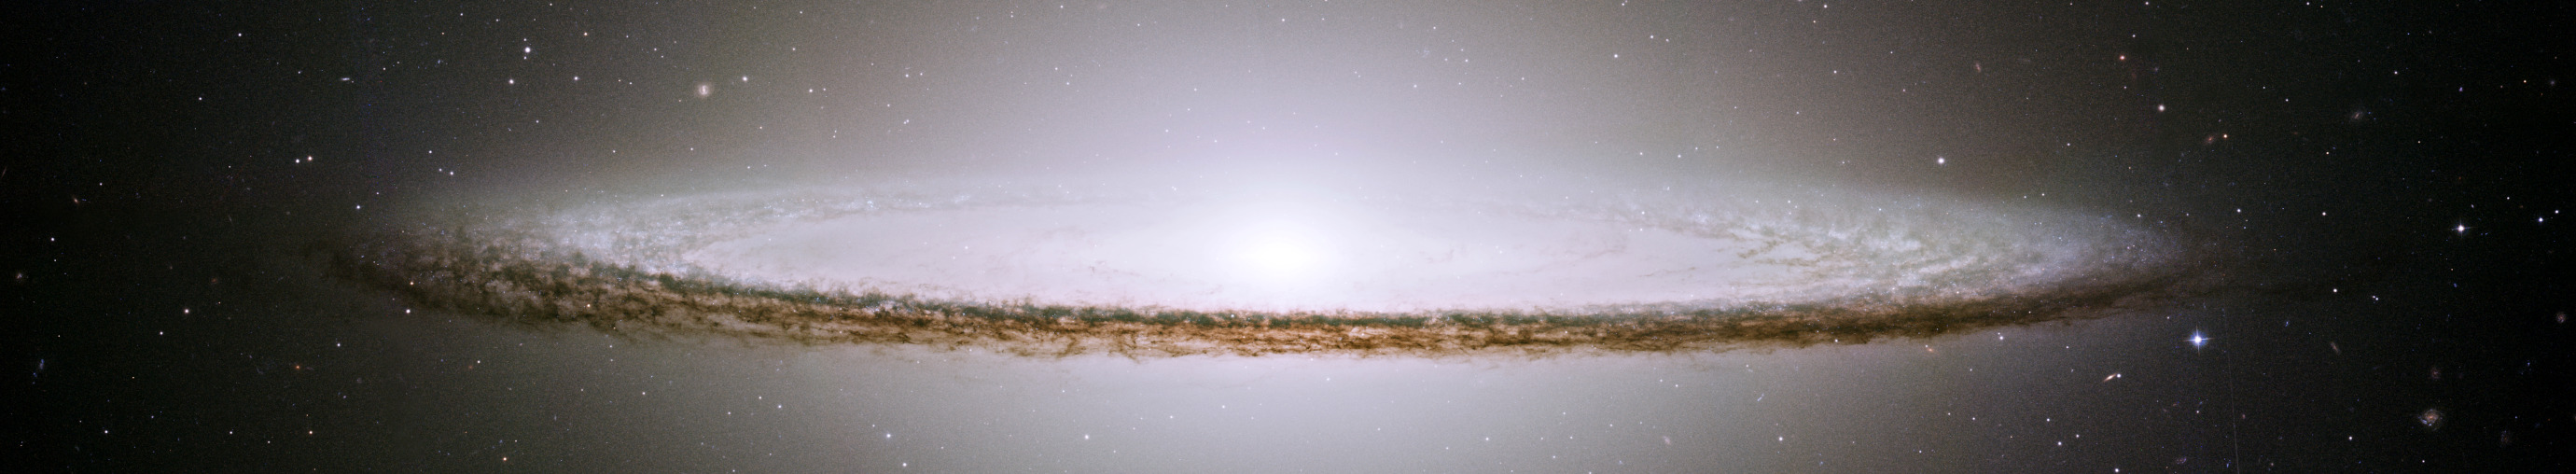
\includegraphics[width=\textwidth]{UWsombrero.jpg}
%  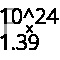
\includegraphics[width=9em]{P.ps}
  %\caption{The Sombrero Galaxy viewed by the Hubble Space Telescope. %(\url{https://some.site}
  %}
  %\Description{A woman and a girl in white dresses sit in an open car.}
\end{figure}
\begin{multicols}{2}
\section{Constants}\begin{align*}%all these ducks in a row go quack
%((299792458)^(−1)) *((6.67430 * (10^-11))^(0)) *((1.6021766 * 10^(-19))^(−1)) *((6.62607015*(10^-34))^(1)) *((1/(2pi))^(0))
\text{SI Avogadro constant } N_A&= 6.02214076×10^{23} \approx {0.012~ kg \over mole ~{{}^{12}C}}\\
\text{Planck constant } h&= 6.62607015 × 10^{-34} kg~m^2~ s^{-1}\\
\text{lightspeed constant } c&=299792458 ~m~s^{-1}\\
\text{electron charge }q_e&=1.602176634 × 10^{-19} \text{Coulombs}\\
\text{gravity constant }G&=6.674 30 × 10^{-11}kg^{-1} m^3 s^{-2}
\end{align*}
$s$ = ``duration of 9192631770 periods of the radiation corresponding to the transition between the two hyperfine levels of the ground state of the cesium 133 atom''\citep{CGPM13} %at gravity equal to sea level.%-``La seconde est la durée de 9192631770 périodes de la radiation correspondant à la transition entre les deux niveaux hyperfins de l´état fondamental de l´atome de césium 133''
to finish the definition of $c$, An international agreement in Paris on Oct. 20 1983 defines the meter as $1\over 299792458$ the distance light travels in a vacuum in 1 second\citep{newspaper_1983}, %\citep{NY Times Nov. 1, 1983, Section C, Page 6 of the National edition with the headline: SCIENCE WATCH}
2018 Codata values of $q_e$, and $G$, come from \citep{RevModPhys.93.025010}.
On May 20, 2019 the values of $\hbar ={{h} \over {2\pi }} $, and $h$, were fixed to their current value along with $N_A$ to the Dalton = ${1 \over 12}$ the mass  ${}^{12}C$ isotope  of Carbon\citep{Horst1}.
\subsection{How the Avogadro constant was measured for the last time}
$N_A$ and $h$ were measured using a incredibly round \& pure ball of $Si^{28}$ and a Kibble balance and the equations basically verbatim from \citep{Horst1}% and \citep{https://doi.org/10.1002/andp.201800308}
Where
${\alpha ^2~m_e~c~/~2~h} = R_\infty$ is the Rydberg constant,
%$\alpha$ is the Fine Structure Constant,
$\sum_{i=28}^{30}x_i~A_r( ^i Si) = A_r(Si)$ average molar mass of a silicon atom in the crystal is calculated using the proportions $x_i$ of the various isotopes $^i Si$,
$V$ is Volume of Silicon Sphere,
$a$ Lattice parameter of the silicon crystal,
$8$ is the number of atoms in an elementary cell of the lattice(cube with edge length a).
$M$ Molar mass of silicon contained in sphere.
$m$  mass of sphere.
$$N= {8~V \over a^3} = \text{Number of atoms in silicon sphere}$$
$$N_A = {M~8~V \over m~a^3}= \text{Avogadro constant}$$
$$m(Si) = {m \over N} = {m~a^3 \over 8 V}= m(e){A_r (Si) \over A_r (e)}$$
$$m(e)= {2~h~R_\infty \over c~\alpha ^2} = {2~\(2\pi~\hbar\) R_\infty \over c~\alpha ^2}$$
$$h={c~ \alpha ^2 \over 2 R_\infty}{m~a^3 \over 8~V}{A_r (e) \over \sum_{i=28}^{30}x_i~A_r( ^i Si)}$$

%\subsection{Rydberg Constant}
%$m_e$ is the rest mass of the electron = 9.1093837015 × 10−31 kg,
%$R_{\infty } = 10973731.568160(21) m−1$
%\begin{align*}
%%(9.1093837015 × 10^−31 ×(0.00729736^2)×3×10^8)/(2×6.62607015×10^−34)=10 981 350.888422
%R_\infty &= {m_e~c~\alpha ^2 \over 2~h}= {m_e~c~\alpha ^2 \over 4~\pi~\hbar}= {m_e~\alpha ^2 \over 4~\pi~m_p~l_p}\\
%{R_\infty ~4~\pi \over c ~m_e}&=  {\alpha ^2 \over \hbar}={t_p \over m_p~l_p^2}\({kg~m~q_e^2 ~10^{-7} \over m_p l_p C^2}\)^2=\\
%\hbar &={m~a^3 \over 8~V}{c~ \alpha ^2 \over 4~\pi}{4~\pi~m_p~l_p \over m_e~\alpha ^2}{A_r (e) \over \sum_{i=28}^{30}x_i~A_r( ^i Si)}\\
%\hbar &={m~a^3 \over 8~V}{m_p~l_p^2 \over t_p ~m_e}{A_r (e) \over \sum_{i=28}^{30}x_i~A_r( ^i Si)}
%\end{align*}

%\section{Acknowledgments}

%\bibliographystyle{plainnat}
\bibliography{math}
\setcounter{table}{0}
\renewcommand{\thetable}{S\arabic{table}}%
\setcounter{figure}{0}
\renewcommand{\thefigure}{S\arabic{figure}}%
\subsection*{Supplementary Materials}
Only reason I found this was for some reason or another I had just looked at $\sqrt{\hbar \alpha}$, and I had Avogadro constant for Stoney-Mass $M_{{\text{S}}} = \sqrt{\hbar ~ \alpha ~c \over G}$ mass popping up in a script I had running with some notes to see how the Planck-Units, and the Stoney-Units\citep{Stoney1883}, baked out the need for certain constants. But when I had left the speed of sound calc to see how the planck units canceled out the Boltzman constant, and the Avogadro constant for $M_S$ also popped up, not exact match but so close I had to do more tests.%The character D in $D_C$ may have something to do with a song by the Rolling Stones. %https://youtu.be/f47TZePukuQ

\end{multicols}
\end{document}
